\subsection{Солнце}
\term{Солнце} --- центральное тело Солнечной системы, в нём сосредоточено 99,866\%  всей массы. Солнце состоит из водорода на 73\% по массе, гелия на 25\% и других элементов с меньшим содержанием: железа, никеля, азота, кислорода, кремния, серы, магния, углерода, неона, кальция, хрома и др.

По спектральной классификации Солнце~--- звезда типа G2V (жёлтый карлик на главной последовательности). Температура поверхности Солнца составляет $5 778$~К, поэтому Солнце светит почти в белом свете, но прямой свет Солнца у поверхности Земли приобретает жёлтый оттенок из-за рассеяния и поглощения коротковолновой части спектра в атмосфере.

Солнце вырабатывает энергию путём термоядерного синтеза. Каждую секунду в ядре около 4~млн.~тонн вещества превращается в лучистую энергию.\\

\term{Строение Солнца.}~~~В центре Солнца находится ядро, радиус которого составляет $150 $ -- $ 180$~тыс.~км, где идут термоядерные реакции. Плотность ядра около $1.5\times 10^5~\text{кг}/\text{м}^3$, а температура в его центре достигает $1.5\times 10^7$~К.

\begin{figure}[h!]
\centering
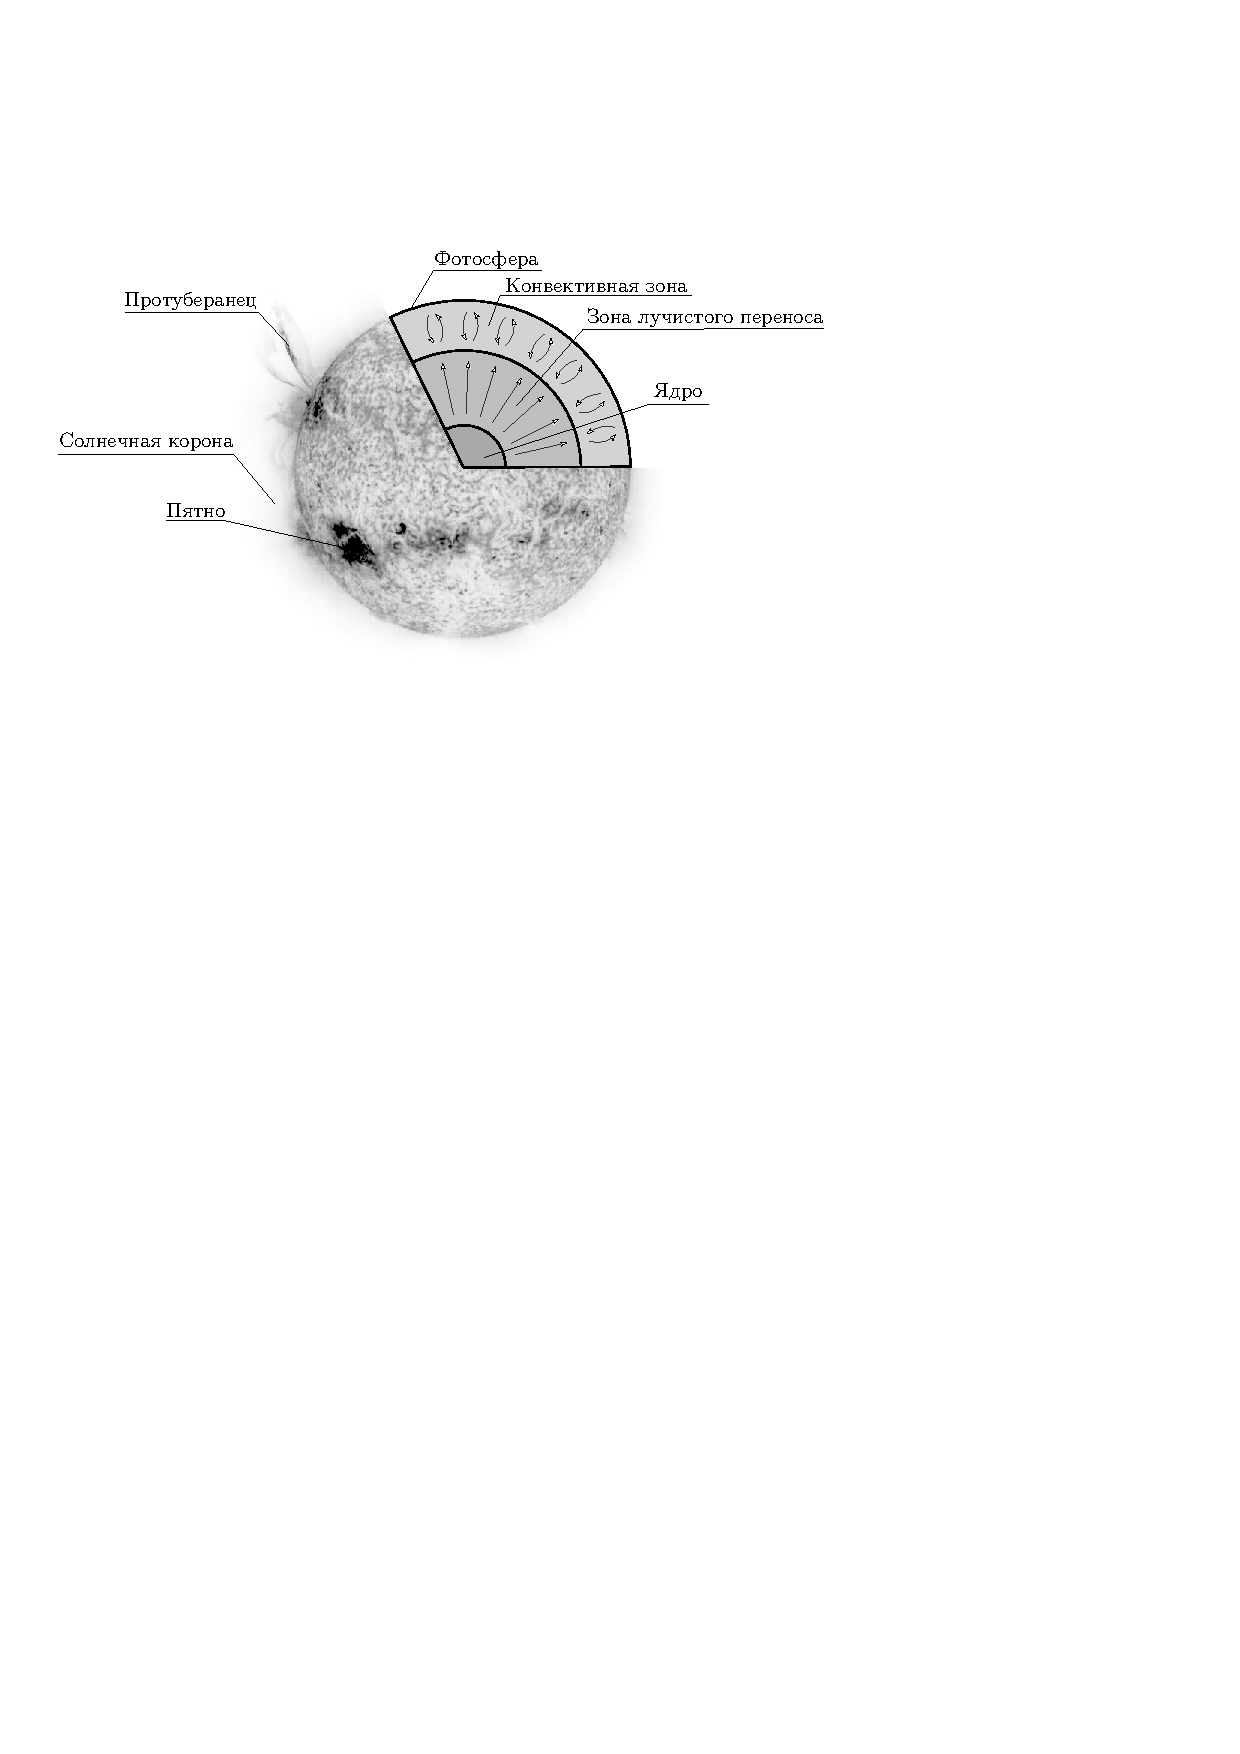
\includegraphics[width=0.8\textwidth]{sun.pdf}
\caption{Строение Солнца. Фотография со спутника1 SOHO в фильтре $H_\alpha$ (негатив)}
\end{figure}
Над ядром, на расстояниях примерно от $0.25 R_\odot$ до $0.7R_\odot$ от его центра, находится \imp{зона лучистого переноса}. В этой зоне перенос энергии происходит главным образом с помощью излучения и поглощения фотонов. Температура в этой зоне лежит в интервале от $2\times10^6$~К сверху до $7\times10^6$~К снизу.

Над зоной лучистого  переноса (радиоактивная зона) находится \imp{конвективная зона}. Это слой толщиной примерно $2\times10^5$~км, в котором перенос энергии к поверхности совершается движением самого вещества. При приближении к поверхности конвективной зоны температура падает до $~5800$~К.

\textit{Фотосфера} --- видимая поверхность Солнца, по которой определяется размер Солнца. Эффективная температура фотосферы $T_\odot =  5778$~К.

\textit{Хромосфера} --- внешняя оболочка Солнца толщиной около 2000 км, окружающая фотосферу. Из хромосферы происходят горячие  выбросы вещества --- \textit{спикулы}. Температура хромосферы увеличивается с высотой до $2\times10^4$~К.

\textit{Солнечная корона} --- последний внешний слой Солнца, который состоит из протуберанцев и энергетических  извержений, образующих солнечный ветер. Средняя температура короны $2 \times 10^6$~К, а в некоторых частях достигает  и $20\times10^6$~К. Столь высокая температура обусловлена процессами, происходящими в магнитном поле звезды. Однако, несмотря на столь высокую температуру, корона видна лишь во время солнечных затмений, так как плотность её очень мала.
  
\term{Вращение Солнца} происходит не твердотельно~--- угловая скорость на разных широтах отличается, при удалении от экватора она уменьшается. Период обращения Солнца на разных широтах можно найти, наблюдая за солнечными пятнами и другими образованиями в фотосфере звезды. На экваторе период вращения составляет 25.05 суток, к полюсу он увеличивается до 34 суток. По наблюдениям за пятнами в течение длительного периода при помощи метода наименьших квадратов можно найти зависимость углового перемещения пятна за сутки от гелиографической широты:
\begin{equation}
\Delta\lambda=14.37^{\circ}-2.7^{\circ}\sin^2\varphi,
\end{equation}
где $\Delta\lambda$~--- угловое перемещение пятна, $\varphi$~--- гелиографическая широта. Данная зависимость верна только для широт $\varphi < 40^\circ$.